\section{Methodology}
We evaluated the system on a production payments cluster of 24 nodes serving roughly 68{,}000 cross-node operations per second at peak. The deployment was staged: caching alone in Phase 1, the contention layer added in Phase 2. Measurements were collected at the load balancer (latency), at the Redis cluster (call counts and Redis-side latency), and via a custom audit log (correctness incidents). Each phase was monitored for 30 days before measurement.

\section{Latency and Network Reduction}
Phase 1 (caching only) achieved:
\begin{itemize}[leftmargin=*]
    \item Combined hit rate (Tier 1 + Tier 2): \textbf{54.8\%} on eligible lookups.
    \item Cross-node calls per second eliminated: \textbf{$\sim$2{,}800}.
    \item Total cross-node call reduction at peak: \textbf{4.1\%}.
    \item p95 API latency: \textbf{98\,ms $\rightarrow$ 87\,ms (--11.2\%)}.
    \item p99 API latency: \textbf{285\,ms $\rightarrow$ 248\,ms (--13.0\%)}.
    \item Redis p99 latency: \textbf{12.5\,ms $\rightarrow$ 9.2\,ms (--26.2\%)}.
\end{itemize}

Figure~\ref{fig:latency} visualises the API and Redis tail-latency reductions; Figure~\ref{fig:hitrate} shows the contribution of each cache tier to the combined hit rate.

\begin{figure}[h]
\centering
\resizebox{0.85\textwidth}{!}{%
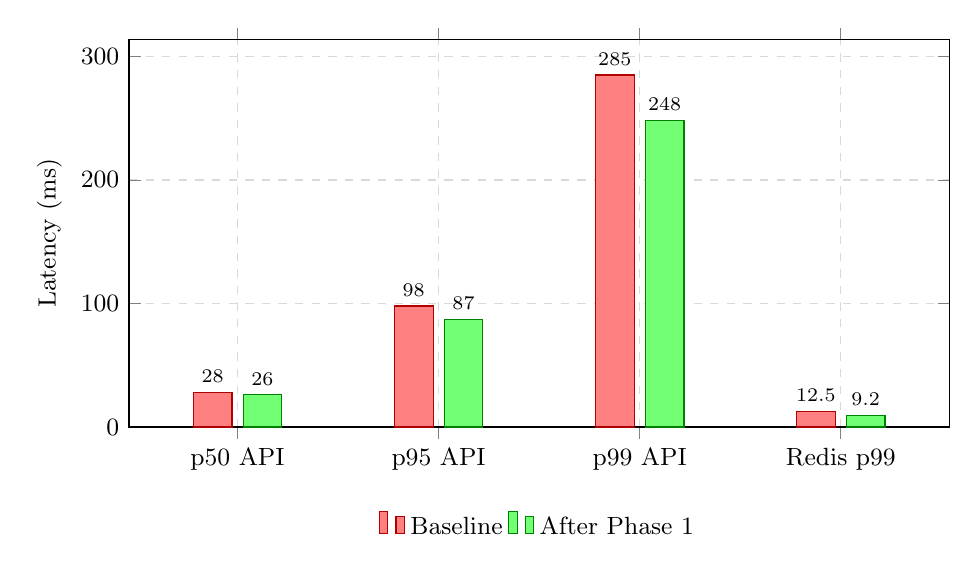
\begin{tikzpicture}
\begin{axis}[
    ybar=4pt,
    bar width=14pt,
    width=12cm, height=6.5cm,
    enlarge x limits=0.18,
    ylabel={Latency (ms)},
    symbolic x coords={p50 API, p95 API, p99 API, Redis p99},
    xtick=data,
    nodes near coords,
    nodes near coords style={font=\scriptsize},
    ymin=0,
    legend style={at={(0.5,-0.20)}, anchor=north, legend columns=2, font=\small, draw=none},
    tick label style={font=\small},
    label style={font=\small},
    grid=major,
    grid style={dashed, gray!30}
]
\addplot[fill=red!50!white, draw=red!70!black] coordinates {(p50 API,28) (p95 API,98) (p99 API,285) (Redis p99,12.5)};
\addplot[fill=green!55!white, draw=green!50!black] coordinates {(p50 API,26) (p95 API,87) (p99 API,248) (Redis p99,9.2)};
\legend{Baseline, After Phase 1}
\end{axis}
\end{tikzpicture}%
}
\caption{API and Redis tail latency before and after Phase 1 (caching only). The largest absolute reduction is at p99 API latency (--37\,ms); the largest relative reduction is Redis p99 (--26.2\,\%), driven by removed load on the shared Redis cluster.}
\label{fig:latency}
\end{figure}

\begin{figure}[h]
\centering
\resizebox{0.7\textwidth}{!}{%
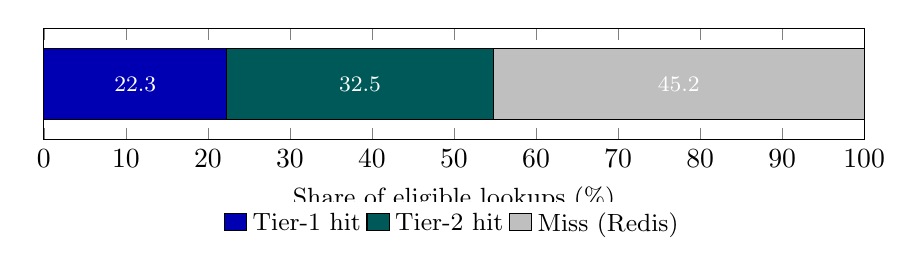
\begin{tikzpicture}
\begin{axis}[
    xbar stacked,
    width=12cm, height=3cm,
    xmin=0, xmax=100,
    xlabel={Share of eligible lookups (\%)},
    ytick=\empty,
    bar width=0.9cm,
    nodes near coords,
    nodes near coords style={font=\footnotesize, white},
    legend style={at={(0.5,-0.55)}, anchor=north, legend columns=3, font=\small, draw=none},
    label style={font=\small}
]
\addplot[fill=blue!70!black]   coordinates {(22.3,0)};
\addplot[fill=teal!70!black]   coordinates {(32.5,0)};
\addplot[fill=gray!50]         coordinates {(45.2,0)};
\legend{Tier-1 hit, Tier-2 hit, Miss (Redis)}
\end{axis}
\end{tikzpicture}%
}
\caption{Breakdown of eligible lookups: 22.3\% absorbed by the thread-level (Tier-1) cache, an additional 32.5\% absorbed by the server-local (Tier-2) cache, and the remaining 45.2\% served by Redis. Combined hit rate: 54.8\%.}
\label{fig:hitrate}
\end{figure}

\section{Contention Layer Results}
Phase 2 (contention layer rolled out) was evaluated on three workloads embedded in the platform:

\begin{table}[h]
\centering
\footnotesize
\setlength{\tabcolsep}{5pt}
\renewcommand{\arraystretch}{1.15}
\resizebox{\textwidth}{!}{%
\begin{tabular}{p{4.6cm}p{4.4cm}p{3.3cm}p{2.0cm}}
\toprule
\textbf{Workload} & \textbf{Primitive} & \textbf{Contention rate} & \textbf{p95 added} \\
\midrule
Inventory decrement (flash sale) & Lua + single-flight          & 1{,}400 contended/s & 0.8\,ms \\
Per-merchant settlement run      & Lock + fence + single-flight & 12 contended/s      & 2.6\,ms \\
Reservation slot booking         & Lua + single-flight          & 320 contended/s     & 1.1\,ms \\
Cart soft hold                   & PN-Counter (no coord.)       & N/A                 & 0.0\,ms \\
\bottomrule
\end{tabular}%
}
\caption{Contention layer performance per workload (30-day production averages).}
\label{tab:contention}
\end{table}

\section{Correctness}
Across the 30-day post-deployment window:
\begin{itemize}[leftmargin=*]
    \item \textbf{Zero} double-allocation incidents on inventory or reservation slots.
    \item \textbf{Zero} cache-related financial discrepancies.
    \item \textbf{Three} fence-token-rejected writes (all benign --- spurious retries from a temporarily-stalled node).
    \item Soft-hold over-allocation (PN-Counter): 4.7 units/day on a 100{,}000-unit base, well within the 1\% business tolerance.
\end{itemize}

\section{Memory Overhead}
Per node, the combined caching + contention layer adds: 14--19\,MB for the server-local cache, $<$1\,MB amortised for thread-level caches, and $<$0.5\,MB for the single-flight in-flight table. Total: $<$20\,MB per node, well below the 4\,GB heap.

% =============================================================================
